\chapter{Experimentální část}
Experimentální studii suspendace v~mechanicky míchané nádobě provedla \citet{pav11} v~rámci své bakalářské práce na Ústavu chemického inženýrství VŠCHT Praha.

\section{Popis experimentu}
\label{chap:exp}
Náplní experimentu bylo měření průběhu suspendace v~systému kapalina-pevná fáze spolu se stanovením doby homogenizace. K~provedení experimentu byla využita válcová nádoba z~plexiskla o~vnitřním průměru $T=\SI{0.29}{\meter}$ s~plochým dnem, jenž byla opatřena čtyřmi radiálními narážkami o~šířce $b=T/10$. Výška plnění nádoby byla zvolena $H=T$. Do této nádoby bylo ve vzdálenosti $C=T/3$ ode dna bylo umístěno šestilopatkové míchadlo se šikmo skloněnými lopatkami (úhel zkosení \SI{45}{\degree}) a celkovým průměrem  $D=T/3$. 
\begin{figure}[h!]
\centering
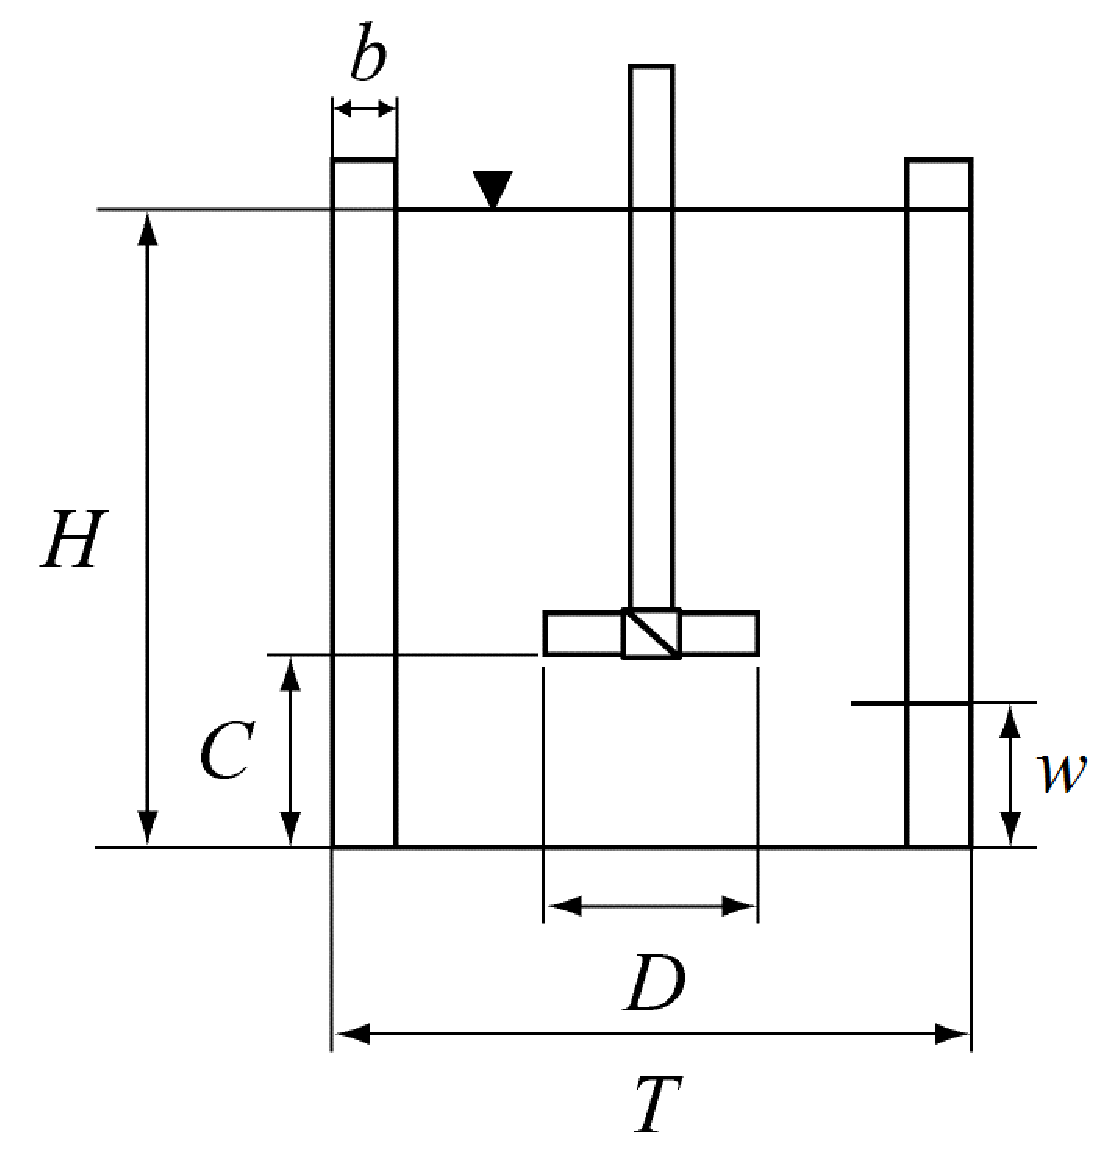
\includegraphics[scale=0.44]{images/mujedit.eps}
\caption{Geometrie experimentu}
\label{fig:nadoba}
\end{figure} 
Detailnější geometrie použitého míchadla je rozkreslena na obrázeku \ref{fig:imp}. Směr rotace hřídele byl volen tak, aby míchadlo vytvářelo axiální proudění proti dnu nádoby. Frekvence jeho otáčení se pohybovala v~intervalu od \SI{3}{\per\second} do \SI{9}{\per\second}, což přibližně odpovídá Reynoldsovu číslu pro míchání ($Re_{M}$) od \num{24500} do \num{73800}.
\begin{figure}[t]
\centering
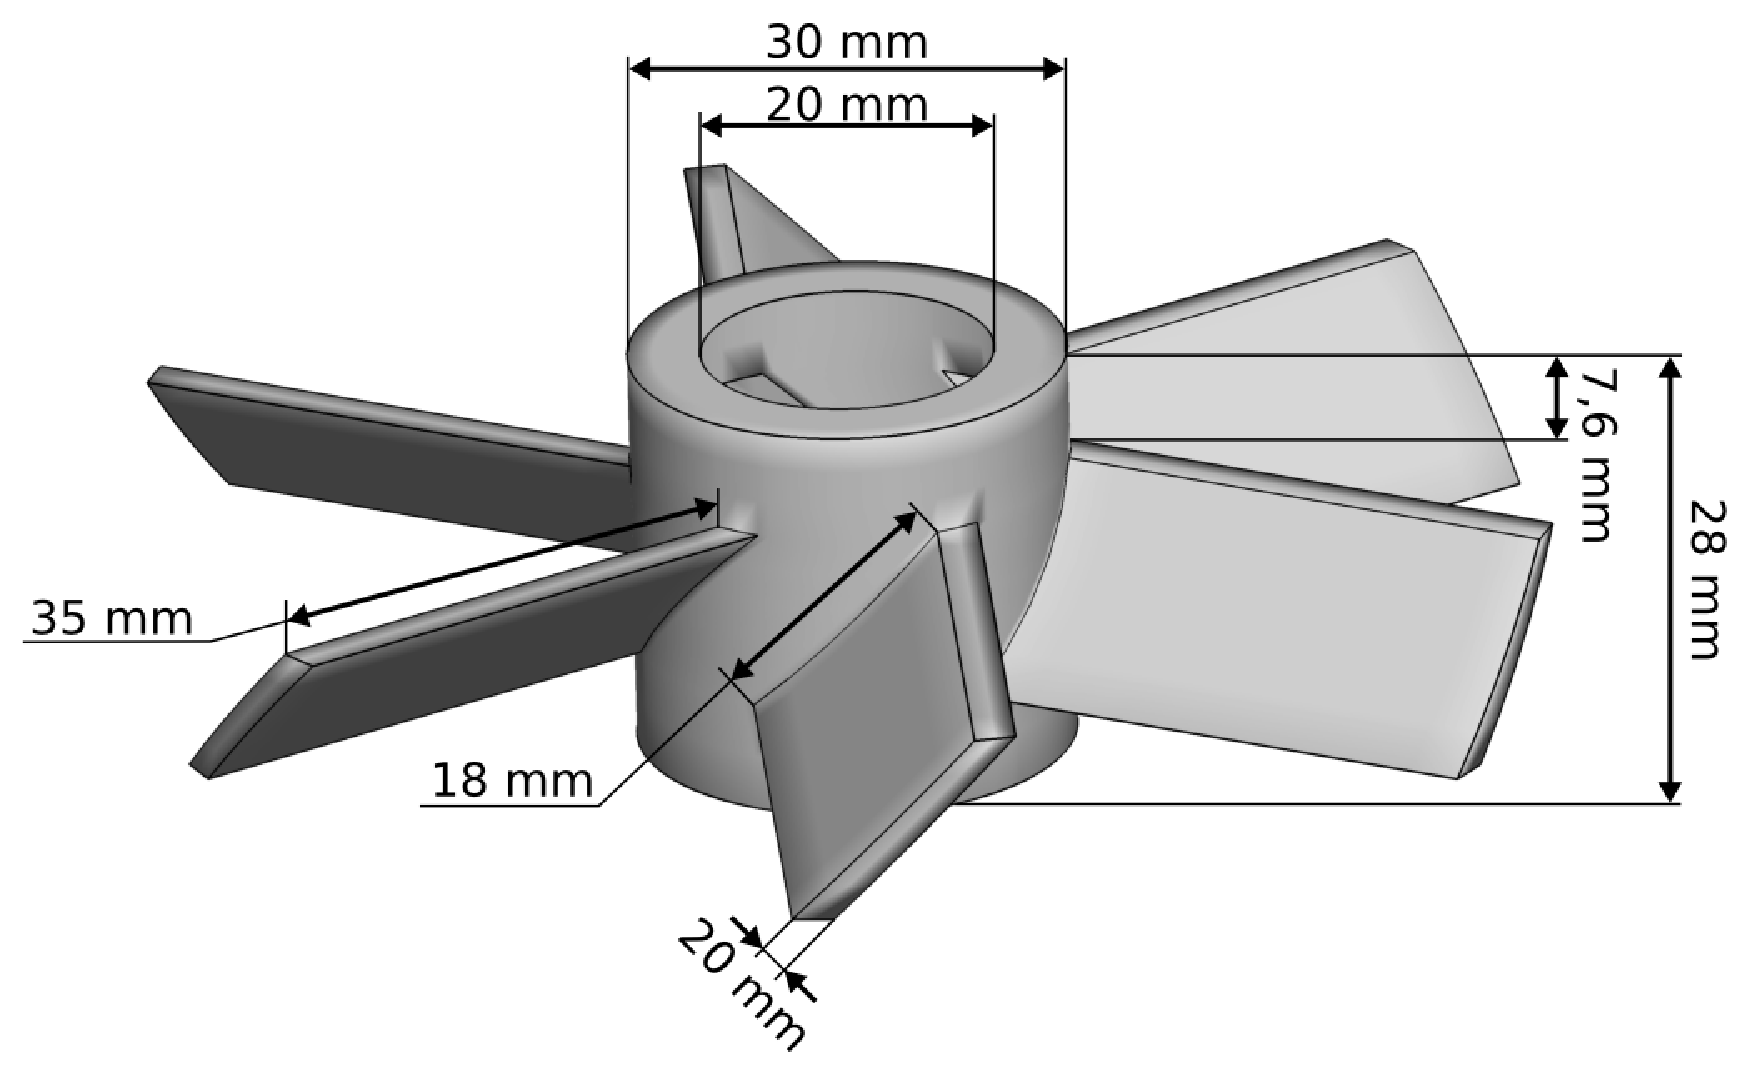
\includegraphics[scale=0.35]{images/imp.eps}
\caption{Geometrie míchadla}
\label{fig:imp}
\end{figure} 

Jako vsádka byla použita voda a polyvinylpyrrolidon (PVP), což je polymer dobře rozpustný ve vodě vykazující newtonovských chováním. Během experimentů byly využity dvě varianty této kapaliny \pvpP{} a \pvpS{} lišící se dynamickou viskozitou (\num{5} resp. \SI{7.5}{\milli\pascal\second}).  Pevnou fázi tvořily červené kuličky z~polyvinylchloridu (PVC) o~průměru \SI{1.02}{\milli\meter}. Vsádka postupně obsahovala 5, 10 a \volproc{15} těchto kuliček. Experimentálně stanovené vlastnosti kapalné a pevné fáze jsou shrnuty v~tabulce \ref{tab:fyzvlast}. 
\begin{table}[h!]
\centering
\caption{Určené vlastnosti kapalné a pevné fáze}
\label{tab:fyzvlast}
\begin{tabular}{llrc}
\toprule
\textbf{Fáze} & \textbf{Veličina} & \textbf{Hodnota} &\textbf{Jednotka} \\
\midrule

voda \\
	& hustota & \num{999.50} & \si{\kilogram\per\cubic\meter} \\
	& dynamická viskozita & \num{1.138} & \si{\milli\pascal\second} \\
\pvpP \\
	& hustota & \num{1011.44} & \si{\kilogram\per\cubic\meter} \\
	& dynamická viskozita & \num{5.050} & \si{\milli\pascal\second} \\
\pvpS \\
	& hustota & \num{1024.18} & \si{\kilogram\per\cubic\meter} \\
	& dynamická viskozita & \num{7.615} & \si{\milli\pascal\second} \\
PVC \\
	& hustota & \num{1136.0} & \si{\kilogram\per\cubic\meter} \\
	& průměr & \num{1.02} & \si{\milli\meter} \\
	& mezerovitost & \num{0.384} & -- \\

\bottomrule
\end{tabular}
\end{table}

Pro určení průběhu homogenizace vsádky byla využita stopovací látka v~podobě chloridu sodného. Jeho roztok o~objemu přibližně \SI{4}{\milli\litre} byl nastříknut na volnou hladinu mezi stěnu nádoby a hřídel míchadla. Koncentrace této látky byla měřena pomocí vodivostní sondy umístěné na opačné straně nádrže ve výšce $w = T/4$ ode dna. Výstupní analogový signál z~čidla o~vzorkovací frekvenci \SI{3}{\hertz} byl po zpracování A/D převodníkem uložen v~připojeném počítači k~dalšímu zpracování. Zaznamenané hodnoty napětí byly následně přepočítány na bezrozměrnou koncentraci $c^{*}$ podle vzorce:    
\begin{equation}
	c^{*} = \frac{c(t) - c_{0}}{c_{\infty} - c_{0}} \approx \frac{U(t) - U_{0}}{U_{\infty} - U_{0}}
	\label{eq:bezkonU}
\end{equation}
přičemž člen $U$ značí hodnotu napětí ve zvoleném čase a význam ostatních symbolů je stejný jako ve vztahu \ref{eq:bezkon}. Doba po které dosáhla fluktuace bezrozměrné koncentrace hodnoty menší než \SI{5}{\percent}, byla považována za dobu homogenizace ($t_{mix}$). 

Během experimentu byly také pořizovaly digitální fotografie míchaného systému lišící se koncentrací pevné fáze, použitou kapalnou vsádkou a rychlostí otáčení míchadla. Získané fotografie byly poté použity k~orientačnímu stanovení výšky vznosu pevné fáze. 
